\chapter{Results}
\label{sec:results}



\begin{figure}
    \centering
    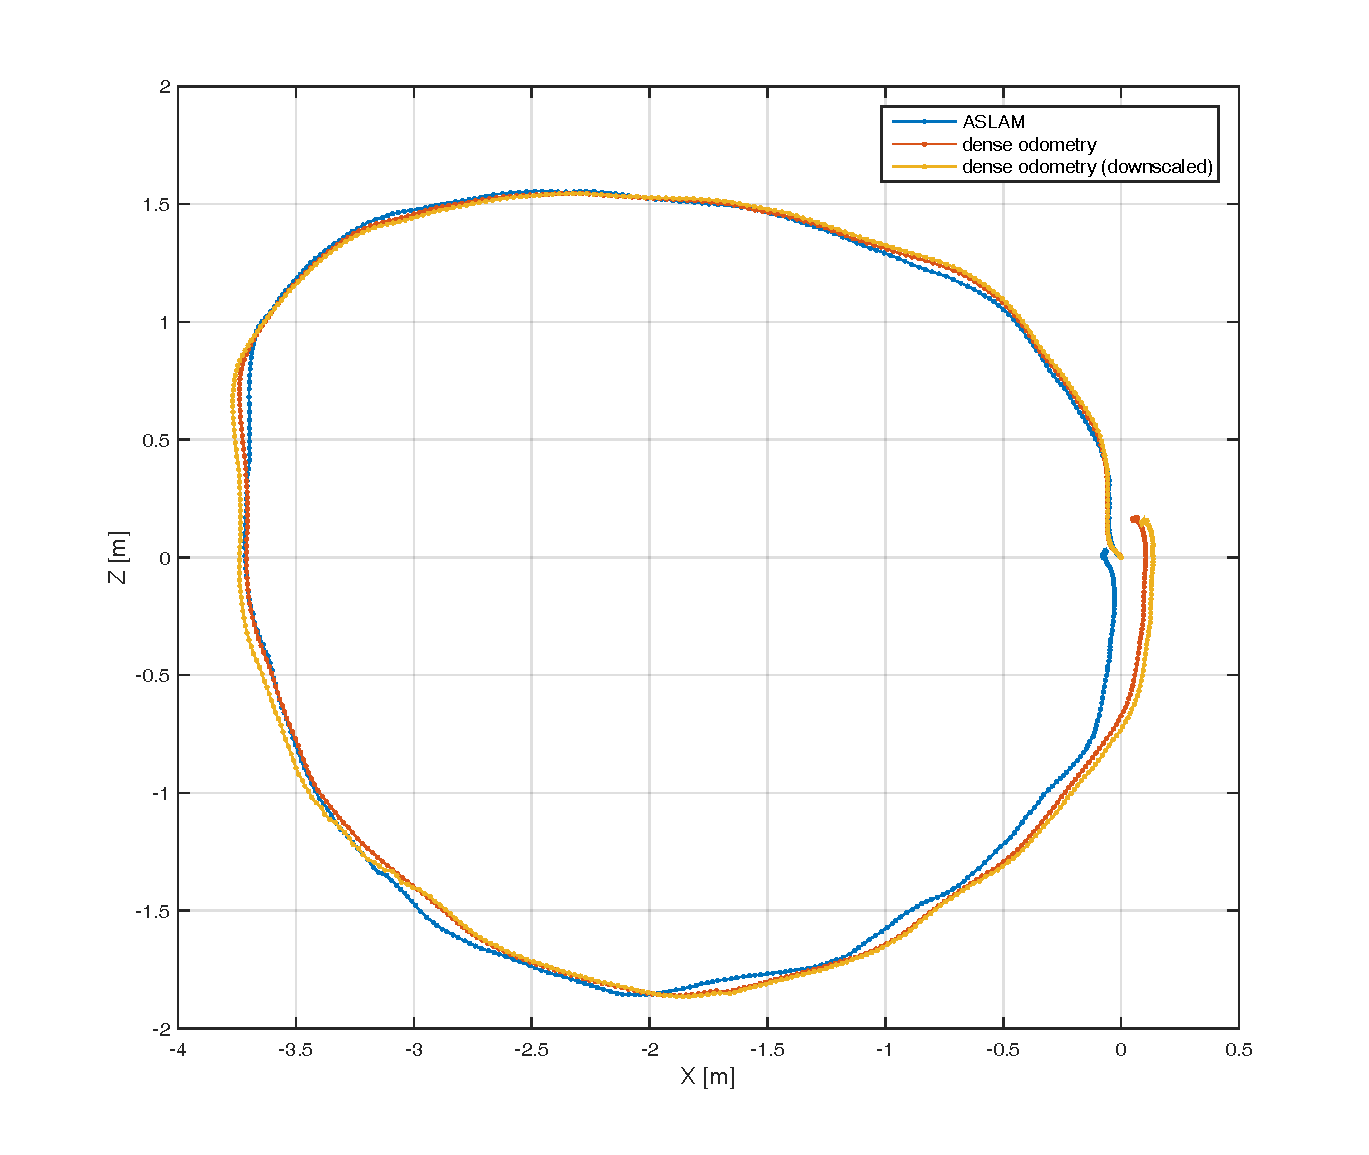
\includegraphics[width=\textwidth]{images/traj_aslam_downscaled.pdf}
    \caption{qualitative comparison of photometric odometry to ASLAM. The red
    trajectory was computed using full image resolution, while the orange one
    only uses $\nicefrac{1}{16}^{th}$ of the available pixels by aborting early in
the image pyramid, thus greatly speeding up runtime performance at negligible
loss of accuracy.}
    \label{fig:trajectory}
\end{figure}

\section{Qualitative Assessment}
\label{sec:results_qualitative}

To assess the quality of photometric approach to visual odometry, a circual
trajectory of an indoor office scene was processed offline with a high quality
SGM from OpenCV and run trough both the very accurate ASLAM algorithm
\cite{leutenegger2013keyframe} and the photometric odometry method described in
this work.

After a traveled distance of about \unit[12]{m} a drift of about \unit[20]{cm}
has been accumulated. On faster trajectories with larger movement between
frames, the Gauss-Newton optimization can diverge resulting in a completely
wrong trajectory.

An important finding, which was already noted in \cite{comport2007odometry}, is
that processing the camera images in their full resolution is not a necessity.
As can be seen in figure~\ref{fig:trajectory}, even using only a twice
downscaled image still results in precise tracking while drastically improving
performance.

Downscaling usually implies filtering and doing so alters the 3D structure. For
this reason, \cite{comport2007odometry} does not downscale the disparity values and
samples them at the full resolution. Though when matching pose on the camera plane
instead of in 3D space, downscaling the disparity values works as well.

It might be worth investigating how much of an effect on performance and
quality downscaling the disparity images has. Disparity values are only read at
integer coordinates and downscaling them might not be worth the runtime
penalty.

\subsection{Keeping Pixel Numbers Stable}

The optimizations described in section~\ref{sec:optimizations} can
substantially reduce the pixel count, so much so that there are not enough for
stable performance. Especially filtering pixels based on their image gradient
as explained in section~\ref{sec:gradient_filtering} requires a well-chosen
threshold, as image gradients depend on the scene. \cite{comport2007odometry}
computes a histogram to select the $N$ best pixels. An easier approach is to
simply restart the current iteration with a lower threshold when the number of
pixels gets too low and increasing it after a step with enough pixels,
therefore implementing a proportional controller as described in
\cite{omaridenseodometry}. The same problem also applies to other optimization
parameters such as the size of the image pyramid.

\section{Timing}
\label{sec:timing}

\begin{figure}
    \centering
    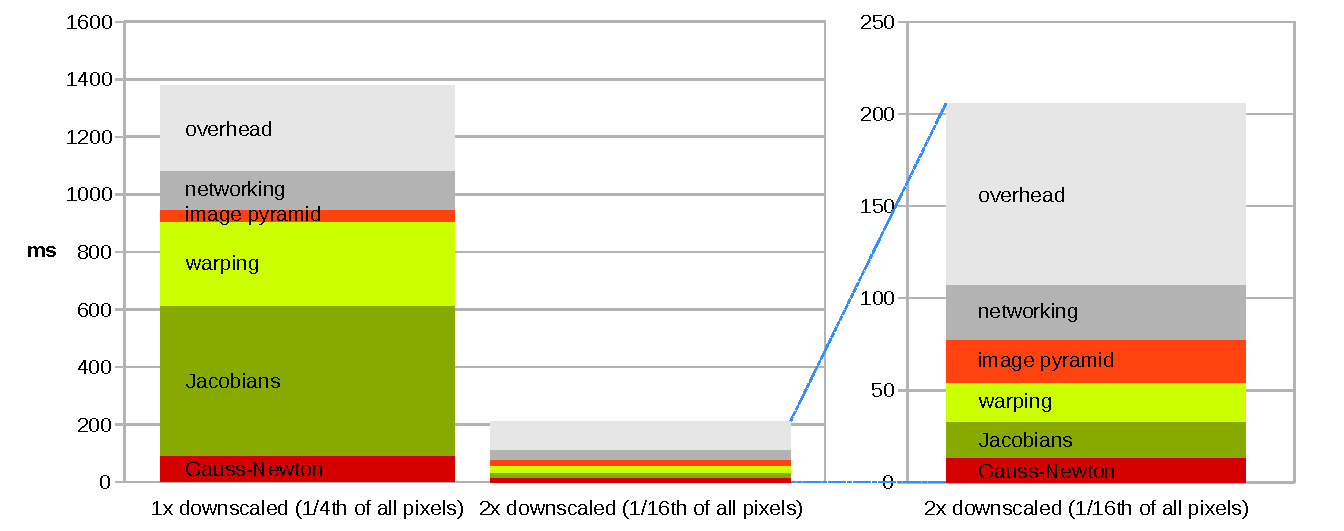
\includegraphics[width=\textwidth]{images/timing.pdf}
    \caption{perfomance breakdown using early abort of the image pyramid}
    \label{fig:timing}
\end{figure}

The different parts of the algorithm have been timed by counting CPU cycles
while running the full photometric odometry on a single ARM core on the
vi-sensor while moving around slowly. The time for the SGM is not shown in
figure~\ref{fig:timing}, as this part is running on the FPGA with the full 30
FPS provided by the cameras.

Using early abort in the image pyramid we can achieve an average run-time
performance of about 5 Hz.
This value not only depends on the algorithm's parameters such as max. pyramid
levels, but also on the scene (more 'dense' environments which provide more
structure converge faster) and on the movement speed. The bigger the steps, the
more iterations are required for convergence, which is counterproductive as a
longer running time implies an even bigger step while moving. This could
potentially be addressed by incorporating integrated acceleration values of an
IMU.

Another important point is that at least half the time is spent on building the
image pyramid, warping pixels and computing the Jacobians. These parts are
highly parallelizable because every pixel is completely independent of each
other. This offers great potential for offloading further work onto the FPGA,
or the second ARM core.
